% !TEX spellcheck = en_US



% ~~~~~~~~~~~~~~~~~~~~~~~~~~~~~~~~~~~~~~~ V
% (NC) 2026 Haluk Bingol
% github.com/halukbingol/LaTeX-Templates
%
% Licensees may copy, distribute, display, and perform the work and make derivative works 
% and remixes based on it only for non-commercial purposes. 
% ~~~~~~~~~~~~~~~~~~~~~~~~~~~~~~~~~~~~~~~ A




% =====================================================================
%  Regular Expressions in Java -- Senior Level: Theory, Engines, Performance and Security
%  ---------------------------------------------------------------------
%  Built on hblib/Template/hblibTemplate.tex with the libraries in ../../hblib/.
%  Programs and their real outputs are in codeoutput/:
%     codeoutput/<Name>.java  a program (classes without main() are only compiled)
%     codeoutput/<Name>.sh    a terminal session, run in a copy of codeoutput/<Name>/
%     codeoutput/<Name>.txt   what it printed, made by:  bash run_examples.sh
% =====================================================================

\documentclass[aspectratio=169,10pt,compress]{beamer}

% ~~~~~~~~~~~~~~~~~~~~~~~~~~~~~~~~~~~~~~~~~~~~~~~~~~~~~~~~~~~~~~~~~ V hblib
	\usepackage{../../hblib/hblibPresentation} % lib presentation: theme, i/N, \hSection, algorithm2e, ...
	\usepackage{../../hblib/hblibCodeoutput} % lib code + output: \lstcode, \lstterminal, ...
	\usepackage{../../hblib/hblibDatastructures} % lib data structures: \hString, \hStack, \hQueue
% ~~~~~~~~~~~~~~~~~~~~~~~~~~~~~~~~~~~~~~~~~~~~~~~~~~~~~~~~~~~~~~~~~ A hblib


% theme, i/N, fonts (T1, lmodern), booktabs, xcolor, array (L{width} columns), listings, tikz,
% algorithm2e (\small captions, \Fn) and the color gitred come from the hblib libraries




% +++++++++++++++++++++++++++++++++++++++ V specific
\DontPrintSemicolon % in algorithms
\newcommand{\win}{\textbf{Windows}}
\newcommand{\mac}{\textbf{macOS}}
\usetikzlibrary{automata,positioning}
% +++++++++++++++++++++++++++++++++++++++ A specific

% ---------------------------------------------------------------------
\title{Regular Expressions in Java}
\subtitle{Senior Level: Theory, Engines, Performance and Security}
\author[Bingol]{Haluk O. Bingol}

\institute[FCIS]{
    Faculty of Computer and Information Sciences\\
    Yeditepe University
}
\date{
	{\tiny \hbTimeStamp}
}

\begin{document}




% ~~~~~~~~~~~~~~~~~~~~~~~~~~~~~~~~~~~~~~ V frm
\begin{frame}[t,fragile]
  \titlepage
\end{frame}
% ~~~~~~~~~~~~~~~~~~~~~~~~~~~~~~~~~~~~~~ A frm




% ~~~~~~~~~~~~~~~~~~~~~~~~~~~~~~~~~~~~~~ V frm
\begin{frame}[t,fragile] \frametitle{Outline}
  \begin{columns}[T]
    \begin{column}{0.48\textwidth}
      \tableofcontents[sections={1-4}, hideallsubsections]
    \end{column}
    \begin{column}{0.48\textwidth}
      \tableofcontents[sections={5-8}, hideallsubsections]
    \end{column}
  \end{columns}
\end{frame}
% ~~~~~~~~~~~~~~~~~~~~~~~~~~~~~~~~~~~~~~ A frm

% ~~~~~~~~~~~~~~~~~~~~~~~~~~~~~~~~~~~~~~ V
\hSection[Theory]{Regular Languages}
% ~~~~~~~~~~~~~~~~~~~~~~~~~~~~~~~~~~~~~~ A




% ~~~~~~~~~~~~~~~~~~~~~~~~~~~~~~~~~~~~~~ V frm
\begin{frame}[t,fragile] \frametitle{Three operations, nothing more}
  A \textbf{regular expression} $r$ over an alphabet $\Sigma$ describes a set of strings $L(r)$:
  \[
  	L(a) = \{a\}, \quad L(r_{1} r_{2}) = L(r_{1})\,L(r_{2}), \quad L(r_{1} \mid r_{2}) = L(r_{1}) \cup L(r_{2}), \quad L(r^{*}) = \bigcup_{k \ge 0} L(r)^{k}
  \]
  \begin{itemize}\small
    \item Everything else is shorthand: $r^{+} = r\,r^{*}$, \ $r? = r \mid \varepsilon$, \ \texttt{[a-c]} $= a \mid b \mid c$, \ $r\{2,3\} = r\,r \mid r\,r\,r$.
    \item Kleene (1956): these are exactly the languages a \textbf{finite automaton} accepts.
    \item A finite automaton has finite memory, so it cannot count without a bound.
    \item Back-references (\texttt{\textbackslash 1}) and look-around are \emph{not} in the theory: Java regexes are more than regular, and pay for it in speed.
  \end{itemize}
\end{frame}
% ~~~~~~~~~~~~~~~~~~~~~~~~~~~~~~~~~~~~~~ A frm




% ~~~~~~~~~~~~~~~~~~~~~~~~~~~~~~~~~~~~~~ V frm
\begin{frame}[t,fragile] \frametitle{A DFA for \texttt{(a|b)*abb}}
  \begin{columns}[T]
    \begin{column}{0.55\textwidth}
      \begin{center}
      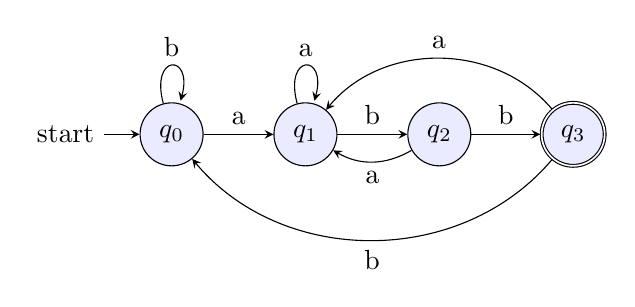
\begin{tikzpicture}[>=stealth, node distance=1.7cm, auto, every state/.style={minimum size=0.8cm, fill=blue!8}]
        \node[state, initial]   (q0)               {$q_{0}$};
        \node[state]            (q1) [right of=q0] {$q_{1}$};
        \node[state]            (q2) [right of=q1] {$q_{2}$};
        \node[state, accepting] (q3) [right of=q2] {$q_{3}$};
        \path[->] (q0) edge [loop above] node {b} (q0)
                       edge              node {a} (q1)
                  (q1) edge [loop above] node {a} (q1)
                       edge              node {b} (q2)
                  (q2) edge              node {b} (q3)
                       edge [bend left]  node {a} (q1)
                  (q3) edge [bend left=50] node {b} (q0)
                       edge [bend right=50, swap] node {a} (q1);
      \end{tikzpicture}
      \end{center}
    \end{column}
    \begin{column}{0.4\textwidth}
      \begin{itemize}\small
        \item One state per ``how much of \texttt{abb} have I just seen''.
        \item Each character: one table look-up. Time $O(n)$ for a text of length $n$, no going back.
        \item State $q_{3}$ accepts: the text ends with \texttt{abb}.
      \end{itemize}
    \end{column}
  \end{columns}
\end{frame}
% ~~~~~~~~~~~~~~~~~~~~~~~~~~~~~~~~~~~~~~ A frm




% ~~~~~~~~~~~~~~~~~~~~~~~~~~~~~~~~~~~~~~ V frm
\begin{frame}[t,fragile] \frametitle{What a finite automaton cannot do}
  \lstcoderightstep[0.62][basicstyle=\ttfamily\tiny][basicstyle=\ttfamily\tiny]{codeoutput/Balanced.java}{Java}{codeoutput/Balanced.txt}

  \vspace{0.2em}
  \small A regex that handles depth $k$ fails at depth $k+1$ (pumping lemma). Brackets, HTML, arithmetic: use a counter, a stack or a parser.
\end{frame}
% ~~~~~~~~~~~~~~~~~~~~~~~~~~~~~~~~~~~~~~ A frm

% ~~~~~~~~~~~~~~~~~~~~~~~~~~~~~~~~~~~~~~ V
\hSection[Engines]{Two Kinds of Engines}
% ~~~~~~~~~~~~~~~~~~~~~~~~~~~~~~~~~~~~~~ A




% ~~~~~~~~~~~~~~~~~~~~~~~~~~~~~~~~~~~~~~ V frm
\begin{frame}[t,fragile] \frametitle{Backtracking: what \texttt{java.util.regex} does}
  \begin{columns}[T]
    \begin{column}{0.56\textwidth}


% +++++++++++++++++++++++++++++++++++++++ V alg
%: -Alg. 
\begin{algorithm}[H]
  \caption{Backtracking match}
  \SetKwFunction{Match}{match}
  \KwIn{a pattern node $p$, the text $s$, a position $i$}
  \KwOut{does $p$, and all that follows it, match at $i$?}
  \lIf{$p$ is the end}{\Return{true}}
  \lIf{$p$ is a character $c$}{\Return{$s_{i} = c$ \textbf{and} \Match{$p.\mathit{next}$, $i+1$}}}
  \If{$p$ is $x \mid y$}{
    \lIf{\Match{$x$, $i$}}{\Return{true}}
    \Return{\Match{$y$, $i$}}\tcp*{go back, try $y$}
  }
  \If{$p$ is $x^{*}$}{
    \lIf(\tcp*[h]{greedy: more first}){\Match{$x\,x^{*}$, $i$}}{\Return{true}}
    \Return{\Match{$p.\mathit{next}$, $i$}}
  }
\end{algorithm}
% +++++++++++++++++++++++++++++++++++++++ A alg

    \end{column}
    \begin{column}{0.4\textwidth}
      \begin{itemize}\small
        \item Easy to extend: groups, \texttt{\textbackslash 1}, look-around, lazy and possessive quantifiers.
        \item Every alternative left untried is a \emph{choice point}; a failure goes back to the last one.
        \item With $k$ nested choices the number of paths can grow like $2^{n}$.
        \item Each recursion is a stack frame: deep repetition can overflow the stack.
      \end{itemize}
    \end{column}
  \end{columns}
\end{frame}
% ~~~~~~~~~~~~~~~~~~~~~~~~~~~~~~~~~~~~~~ A frm




% ~~~~~~~~~~~~~~~~~~~~~~~~~~~~~~~~~~~~~~ V frm
\begin{frame}[t,fragile] \frametitle{Automaton simulation: RE2, RE2/J, Go, Rust}
  \begin{columns}[T]
    \begin{column}{0.56\textwidth}


% +++++++++++++++++++++++++++++++++++++++ V alg
%: -Alg. 
\begin{algorithm}[H]
  \caption{NFA simulation (Thompson)}
  \KwIn{an NFA with start state $q_{0}$ and transitions $\delta$, a text $s_{1} \dots s_{n}$}
  $S \leftarrow \mathrm{closure}(\{q_{0}\})$\tcp*{states reachable by $\varepsilon$}
  \For{$i \leftarrow 1$ \KwTo $n$}{
    $S \leftarrow \mathrm{closure}(\{\, q' : q \in S,\ q' \in \delta(q, s_{i}) \,\})$\;
  }
  \Return{$S$ contains an accepting state}
\end{algorithm}
% +++++++++++++++++++++++++++++++++++++++ A alg

    \end{column}
    \begin{column}{0.4\textwidth}
      \begin{itemize}\small
        \item All choices are followed \emph{at the same time}: a set of at most $m$ states.
        \item Time $O(m \cdot n)$ for a pattern of size $m$: never exponential.
        \item The price: no back-references, no look-around.
        \item Backtracking engines: Java, Perl, PCRE, Python, JavaScript. Automaton engines: RE2, RE2/J, Go, Rust.
      \end{itemize}
    \end{column}
  \end{columns}
\end{frame}
% ~~~~~~~~~~~~~~~~~~~~~~~~~~~~~~~~~~~~~~ A frm

% ~~~~~~~~~~~~~~~~~~~~~~~~~~~~~~~~~~~~~~ V
\hSection[ReDoS]{Catastrophic Backtracking (ReDoS)}
% ~~~~~~~~~~~~~~~~~~~~~~~~~~~~~~~~~~~~~~ A




% ~~~~~~~~~~~~~~~~~~~~~~~~~~~~~~~~~~~~~~ V frm
\begin{frame}[t,fragile] \frametitle{A real pattern that gets slow}
  \lstcoderightstep[0.58][basicstyle=\ttfamily\tiny][basicstyle=\ttfamily\tiny]{codeoutput/Csv.java}{Java}{codeoutput/Csv.txt}

  \vspace{0.2em}
  \small ``Is field 12 a \texttt{P}?'' On a line with no \texttt{P}, \texttt{.*?} may also swallow commas: the engine tries every way to cut the line into 11 pieces. \texttt{[\textasciicircum ,]*} can cut it only one way. Times vary; the growth does not.
\end{frame}
% ~~~~~~~~~~~~~~~~~~~~~~~~~~~~~~~~~~~~~~ A frm




% ~~~~~~~~~~~~~~~~~~~~~~~~~~~~~~~~~~~~~~ V frm
\begin{frame}[t,fragile] \frametitle{Java remembers, but not everything}
  \lstcoderightstep[0.56][basicstyle=\ttfamily\tiny][basicstyle=\ttfamily\tiny]{codeoutput/Memo.java}{Java}{codeoutput/Memo.txt}

  \vspace{0.2em}
  \small The JDK caches failed attempts of greedy loops: \texttt{(a+)+b} is only quadratic (twice $n$, about $4\times$ the time). With \texttt{\textbackslash 1} the cache cannot help: every $+2$ in $n$, about $4\times$ the time: exponential.
\end{frame}
% ~~~~~~~~~~~~~~~~~~~~~~~~~~~~~~~~~~~~~~ A frm




% ~~~~~~~~~~~~~~~~~~~~~~~~~~~~~~~~~~~~~~ V frm
\begin{frame}[t,fragile] \frametitle{Avoiding ReDoS}
  \begin{itemize}\small
    \item \textbf{No overlapping choices}: in \texttt{(.*?,)\{11\}} the dot and the comma overlap; \texttt{[\textasciicircum ,]*,} does not. Avoid \texttt{(x+)+}, \texttt{(x|x)*}, \texttt{(\textbackslash w|\textbackslash d)+}.
    \item \textbf{Possessive and atomic}: \texttt{[\textasciicircum ,]*+,} and \texttt{(?>\dots)} throw the choice points away.
    \item \textbf{Anchor}: \texttt{\textasciicircum\dots\$} with \texttt{matches()}; no unanchored \texttt{.*} at the start of \texttt{find()}.
    \item \textbf{Limit the input}: check the length \emph{before} matching (a 100-character name field needs no 10\,MB input).
    \item \textbf{Limit the time}: a deadline (next section), or an automaton engine (RE2/J).
    \item \textbf{Test the failing case}: slowness shows when the match \emph{fails}; time the worst input in a unit test.
    \item Never compile a pattern that a user typed without limits (see Security).
  \end{itemize}
\end{frame}
% ~~~~~~~~~~~~~~~~~~~~~~~~~~~~~~~~~~~~~~ A frm

% ~~~~~~~~~~~~~~~~~~~~~~~~~~~~~~~~~~~~~~ V
\hSection[Stack]{Stack Overflow}
% ~~~~~~~~~~~~~~~~~~~~~~~~~~~~~~~~~~~~~~ A




% ~~~~~~~~~~~~~~~~~~~~~~~~~~~~~~~~~~~~~~ V frm
\begin{frame}[t,fragile] \frametitle{Long input, deep recursion}
  \lstcoderightstep[0.56][basicstyle=\ttfamily\tiny][basicstyle=\ttfamily\tiny]{codeoutput/Overflow.java}{Java}{codeoutput/Overflow.txt}

  \vspace{0.2em}
  \small A group with \texttt{|} repeated 40\,000 times recurses 40\,000 deep. A character class (\texttt{[ab]*}) or a group without a choice is a simple loop. A bigger stack (\texttt{java -Xss64m}) only moves the limit.
\end{frame}
% ~~~~~~~~~~~~~~~~~~~~~~~~~~~~~~~~~~~~~~ A frm

% ~~~~~~~~~~~~~~~~~~~~~~~~~~~~~~~~~~~~~~ V
\hSection[Defences]{Time Limits and RE2/J}
% ~~~~~~~~~~~~~~~~~~~~~~~~~~~~~~~~~~~~~~ A




% ~~~~~~~~~~~~~~~~~~~~~~~~~~~~~~~~~~~~~~ V frm
\begin{frame}[t,fragile] \frametitle{A deadline inside \texttt{charAt}}
  \begin{columns}[T]
    \begin{column}{0.49\textwidth}
      \lstcode[basicstyle=\ttfamily\tiny, lastline=14]{codeoutput/Deadline.java}{Java}
    \end{column}
    \begin{column}{0.49\textwidth}
      \lstcode[basicstyle=\ttfamily\tiny, firstline=15, firstnumber=15]{codeoutput/Deadline.java}{Java}
    \end{column}
  \end{columns}
\end{frame}
% ~~~~~~~~~~~~~~~~~~~~~~~~~~~~~~~~~~~~~~ A frm




% ~~~~~~~~~~~~~~~~~~~~~~~~~~~~~~~~~~~~~~ V frm
\begin{frame}[t,fragile] \frametitle{A deadline inside \texttt{charAt}: the run}
  \begin{columns}[T]
    \begin{column}{0.4\textwidth}
      \lstoutput[basicstyle=\ttfamily\scriptsize]{codeoutput/Deadline.txt}
    \end{column}
    \begin{column}{0.56\textwidth}
      \begin{itemize}\small
        \item Short input: the normal answer, \texttt{false}, long before the deadline.
        \item 40 characters: exponential; after 100\,ms the next \texttt{charAt} throws.
        \item \texttt{Matcher} cannot be interrupted, but it reads the text only through \texttt{CharSequence.charAt}: the clock is checked there.
        \item Choose a limit far above the normal case; log every timeout.
      \end{itemize}
    \end{column}
  \end{columns}
\end{frame}
% ~~~~~~~~~~~~~~~~~~~~~~~~~~~~~~~~~~~~~~ A frm




% ~~~~~~~~~~~~~~~~~~~~~~~~~~~~~~~~~~~~~~ V frm
\begin{frame}[t,fragile] \frametitle{RE2/J: linear time}
  \begin{columns}[T]
    \begin{column}{0.49\textwidth}
      \lstcode[basicstyle=\ttfamily\tiny, lastline=13]{codeoutput/Re2/Re2.java}{Java}
    \end{column}
    \begin{column}{0.49\textwidth}
      \lstcode[basicstyle=\ttfamily\tiny, firstline=14, firstnumber=14]{codeoutput/Re2/Re2.java}{Java}
    \end{column}
  \end{columns}
\end{frame}
% ~~~~~~~~~~~~~~~~~~~~~~~~~~~~~~~~~~~~~~ A frm




% ~~~~~~~~~~~~~~~~~~~~~~~~~~~~~~~~~~~~~~ V frm
\begin{frame}[t,fragile] \frametitle{RE2/J: the run}
  \begin{columns}[T]
    \begin{column}{0.52\textwidth}
      \lstterminal[basicstyle=\ttfamily\tiny]{codeoutput/Re2.txt}
    \end{column}
    \begin{column}{0.44\textwidth}
      \begin{itemize}\small
        \item The CSV pattern (28 fields): RE2/J is fast, \texttt{java.util.regex} is not.
        \item \texttt{(a|b)*} on 40\,000 characters: no recursion, no stack overflow.
        \item Back-references are refused when the pattern is compiled.
        \item Same API (\texttt{Pattern}, \texttt{Matcher}), other package: \texttt{com.google.re2j}.
      \end{itemize}
    \end{column}
  \end{columns}
\end{frame}
% ~~~~~~~~~~~~~~~~~~~~~~~~~~~~~~~~~~~~~~ A frm




% ~~~~~~~~~~~~~~~~~~~~~~~~~~~~~~~~~~~~~~ V frm
\begin{frame}[t,fragile] \frametitle{Getting RE2/J}
  \begin{itemize}\small
    \item Google's Java port of RE2: \texttt{com.google.re2j:re2j}, version 1.7 (the latest on Maven Central); the same \texttt{Pattern}/\texttt{Matcher} API, other package.
    \item Maven: \texttt{<dependency>} with group \texttt{com.google.re2j}, artifact \texttt{re2j} (not run here: no internet).
    \item By hand: download \texttt{re2j-1.7.jar} into the project folder, then:
  \end{itemize}
  \begin{columns}[T]
    \begin{column}{0.48\textwidth}
      \begin{block}{Windows (Command Prompt)}


% +++++++++++++++++++++++++++++++++++++++ V lst
%: -Lst.
\begin{lstlisting}[style=codesnippet, language={}, basicstyle=\ttfamily\scriptsize]
javac -cp re2j-1.7.jar Re2.java
java -cp re2j-1.7.jar;. Re2
\end{lstlisting}
% +++++++++++++++++++++++++++++++++++++++ A lst


      \end{block}
    \end{column}
    \begin{column}{0.48\textwidth}
      \begin{block}{macOS (Terminal)}


% +++++++++++++++++++++++++++++++++++++++ V lst
%: -Lst.
\begin{lstlisting}[style=codesnippet, language=bash, basicstyle=\ttfamily\scriptsize]
javac -cp re2j-1.7.jar Re2.java
java -cp re2j-1.7.jar:. Re2
\end{lstlisting}
% +++++++++++++++++++++++++++++++++++++++ A lst


      \end{block}
    \end{column}
  \end{columns}

  \small The class path separator: \texttt{;} on Windows, \texttt{:} on macOS and Linux. The run above used Debian's \texttt{libre2j-java} (1.7).
\end{frame}
% ~~~~~~~~~~~~~~~~~~~~~~~~~~~~~~~~~~~~~~ A frm

% ~~~~~~~~~~~~~~~~~~~~~~~~~~~~~~~~~~~~~~ V
\hSection[Security]{Regex Injection}
% ~~~~~~~~~~~~~~~~~~~~~~~~~~~~~~~~~~~~~~ A




% ~~~~~~~~~~~~~~~~~~~~~~~~~~~~~~~~~~~~~~ V frm
\begin{frame}[t,fragile] \frametitle{User text inside a pattern}
  \lstcoderightstep[0.58][basicstyle=\ttfamily\tiny][basicstyle=\ttfamily\tiny]{codeoutput/Injection.java}{Java}{codeoutput/Injection.txt}

  \vspace{0.2em}
  \small User text in a pattern is code: \texttt{.} matched \texttt{x}. \texttt{Pattern.quote} wraps it in \texttt{\textbackslash Q\dots\textbackslash E}; \texttt{Matcher.quoteReplacement} protects \texttt{\$} and \texttt{\textbackslash} in a replacement. A user-written pattern can also be a ReDoS.
\end{frame}
% ~~~~~~~~~~~~~~~~~~~~~~~~~~~~~~~~~~~~~~ A frm

% ~~~~~~~~~~~~~~~~~~~~~~~~~~~~~~~~~~~~~~ V
\hSection[Limits]{When Not to Use a Regex}
% ~~~~~~~~~~~~~~~~~~~~~~~~~~~~~~~~~~~~~~ A




% ~~~~~~~~~~~~~~~~~~~~~~~~~~~~~~~~~~~~~~ V frm
\begin{frame}[t,fragile] \frametitle{HTML is not regular}
  \lstcoderightstep[0.6][basicstyle=\ttfamily\tiny][basicstyle=\ttfamily\scriptsize]{codeoutput/Tags.java}{Java}{codeoutput/Tags.txt}

  \vspace{0.2em}
  \small Nested tags and attributes break it: the second line found \texttt{x<b>y}, the third nothing. Use an HTML parser (e.g.\ jsoup); for JSON, XML, CSV with quotes, Java source: their parsers.
\end{frame}
% ~~~~~~~~~~~~~~~~~~~~~~~~~~~~~~~~~~~~~~ A frm




% ~~~~~~~~~~~~~~~~~~~~~~~~~~~~~~~~~~~~~~ V frm
\begin{frame}[t,fragile] \frametitle{Regex or not?}
  \begin{center}\footnotesize
  \begin{tabular}{@{}L{0.36\textwidth}L{0.58\textwidth}@{}}
    \toprule
    \textbf{task}                          & \textbf{better tool} \\
    \midrule
    nested structure (brackets, HTML, JSON) & a parser: jsoup, Jackson, a recursive-descent parser \\
    e-mail ``valid?''                       & a simple check (\texttt{.+@.+\textbackslash..+}), then send a confirmation mail \\
    dates                                   & \texttt{LocalDate.parse} with a \texttt{DateTimeFormatter} \\
    numbers                                 & \texttt{Integer.parseInt}, \texttt{new BigDecimal(s)} in \texttt{try} \\
    one fixed separator                     & \texttt{String.indexOf}, \texttt{split} with one character \\
    CSV with quoted fields                  & a CSV library \\
    tokens of a small language              & a regex per token is fine; the grammar needs a parser \\
    \bottomrule
  \end{tabular}
  \end{center}
\end{frame}
% ~~~~~~~~~~~~~~~~~~~~~~~~~~~~~~~~~~~~~~ A frm

% ~~~~~~~~~~~~~~~~~~~~~~~~~~~~~~~~~~~~~~ V
\hSection[Summary]{Summary}
% ~~~~~~~~~~~~~~~~~~~~~~~~~~~~~~~~~~~~~~ A




% ~~~~~~~~~~~~~~~~~~~~~~~~~~~~~~~~~~~~~~ V frm
\begin{frame}[t,fragile] \frametitle{Summary}
  \begin{itemize}\small
    \item Regular expressions = finite automata; they cannot count without a bound.
    \item \texttt{java.util.regex} backtracks: rich features, but the time can explode and deep repetition can overflow the stack.
    \item ReDoS comes from overlapping choices; it shows on \emph{failing} input. Fix the pattern: negated classes, possessive and atomic parts, anchors.
    \item Defend in depth: input length limits, a deadline in \texttt{charAt}, or RE2/J for patterns from outside.
    \item \texttt{Pattern.quote} and \texttt{Matcher.quoteReplacement} for any user text.
    \item Nested formats need parsers, not regexes.
  \end{itemize}
\end{frame}
% ~~~~~~~~~~~~~~~~~~~~~~~~~~~~~~~~~~~~~~ A frm




% ~~~~~~~~~~~~~~~~~~~~~~~~~~~~~~~~~~~~~~ V frm
\begin{frame}[t,fragile] \frametitle{Projects}
  \begin{enumerate}\small
    \item \textbf{A tiny engine}: implement the backtracking algorithm for \texttt{a}, \texttt{.}, \texttt{*}, \texttt{|}, \texttt{()}, then Thompson's NFA simulation; compare their times on \texttt{(a*)*b}.
    \item \textbf{ReDoS hunter}: find nested or overlapping quantifiers in all \texttt{Pattern.compile} calls of a project (a regex over regexes!) and time each on a failing input.
    \item \textbf{Safe matcher}: a library \texttt{SafeRegex.matches(pattern, text, millis)} using the deadline \texttt{CharSequence}, with JUnit tests for the timeout.
    \item \textbf{RE2/J or not}: run all patterns of a project on RE2/J; list those it rejects and why.
    \item \textbf{Tokenizer}: a lexer for arithmetic with named groups and \texttt{\textbackslash G}, plus a recursive-descent parser for the brackets.
  \end{enumerate}
\end{frame}
% ~~~~~~~~~~~~~~~~~~~~~~~~~~~~~~~~~~~~~~ A frm




% ~~~~~~~~~~~~~~~~~~~~~~~~~~~~~~~~~~~~~~ V frm
\begin{frame}[t,fragile]
	\begin{center}
		\vspace{4cm}
		\hRemark{\Huge Questions?}
	\end{center}
\end{frame}
% ~~~~~~~~~~~~~~~~~~~~~~~~~~~~~~~~~~~~~~ A frm



\end{document}
